\documentclass[tikz,border=5pt]{standalone}

\usepackage{fontspec}
\usepackage{unicode-math}
\usepackage{pgfplots}

\pgfplotsset{compat=1.18}

% Compile with LuaLaTeX or XeLaTeX.
\setmainfont{STIX Two Text}
\setmathfont{STIX Two Math}

\colorlet{functioncolor}{red!75!black}
\colorlet{rulecolor}{blue!65!black}

\begin{document}

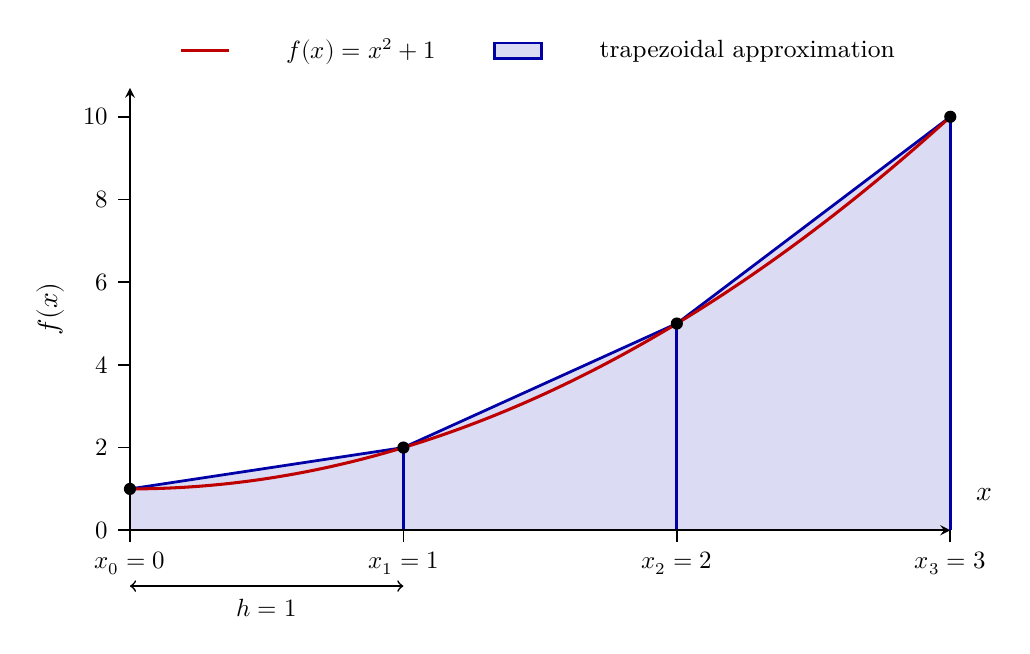
\begin{tikzpicture}

  \begin{axis}[
      width=12cm,
      height=7.2cm,
      xmin=0, xmax=3,
      ymin=0, ymax=10.7,
      axis lines=left,
      axis on top,
      axis line style={black, semithick},
      tick align=outside,
      tick style={black, semithick},
      xlabel={\(x\)},
      ylabel={\(f(x)\)},
      xlabel style={at={(axis description cs:1.02,0.08)}, anchor=west},
      xtick={0,1,2,3},
      xticklabels={\(x_0=0\),\(x_1=1\),\(x_2=2\),\(x_3=3\)},
      ytick={0,2,4,6,8,10},
      tick label style={font=\small},
      label style={font=\normalsize},
      legend style={
          at={(0.5,1.03)},
          anchor=south,
          draw=none,
          fill=none,
          font=\small,
          legend columns=-1,
          column sep=0.65cm,
        },
      clip=false,
    ]

    % Trapezoids, drawn first so the function remains visible.
    \fill[rulecolor!14]
    (axis cs:0,0) -- (axis cs:0,1) -- (axis cs:1,2) -- (axis cs:1,0) -- cycle;
    \fill[rulecolor!14]
    (axis cs:1,0) -- (axis cs:1,2) -- (axis cs:2,5) -- (axis cs:2,0) -- cycle;
    \fill[rulecolor!14]
    (axis cs:2,0) -- (axis cs:2,5) -- (axis cs:3,10) -- (axis cs:3,0) -- cycle;

    % Piecewise-linear approximation through the endpoint values.
    \draw[rulecolor, line width=1pt]
    (axis cs:0,1) -- (axis cs:1,2) -- (axis cs:2,5) -- (axis cs:3,10);
    \draw[rulecolor, line width=1pt] (axis cs:0,0) -- (axis cs:0,1);
    \draw[rulecolor, line width=1pt] (axis cs:1,0) -- (axis cs:1,2);
    \draw[rulecolor, line width=1pt] (axis cs:2,0) -- (axis cs:2,5);
    \draw[rulecolor, line width=1pt] (axis cs:3,0) -- (axis cs:3,10);

    % The integrand.
    \addplot[
      domain=0:3,
      samples=150,
      functioncolor,
      line width=1.1pt,
      forget plot,
    ] {x^2+1};

    % Endpoint evaluation points.
    \fill[black] (axis cs:0,1) circle (2.2pt);
    \fill[black] (axis cs:1,2) circle (2.2pt);
    \fill[black] (axis cs:2,5) circle (2.2pt);
    \fill[black] (axis cs:3,10) circle (2.2pt);

    % One dimension line to identify the uniform spacing.
    \draw[<->, semithick]
    (axis cs:0,-1.35) -- (axis cs:1,-1.35)
    node[midway, below=1pt, font=\small] {\(h=1\)};

    % Two-item legend, shared in style with the midpoint figure.
    \addlegendimage{functioncolor, line width=1.1pt}
    \addlegendentry{\(f(x)=x^2+1\)}
    \addlegendimage{area legend, draw=rulecolor, fill=rulecolor!14, line width=1pt}
    \addlegendentry{trapezoidal approximation}

  \end{axis}

\end{tikzpicture}

\end{document}
